\chapter{Experiments and Benchmarking}
\label{chp:contrib_ResultsDiscussion}

In the following sections, we present the results obtained with the modified \ac{ABA} algorithm, the reinforcement learning framework, and the robot codesign process. In particular, we present the results obtained with the modified \ac{ABA} algorithm in \cref{sec:results_fd_aba}, supported by the theory presented in \cref{chp:contrib_ABA},
and the results obtained with the robot codesign process in \cref{sec:codesign_results}, which are the outcomes of the work presented in \cref{chp:contrib_CodesignRL}.

\section{Modified Forward Dynamics Benchmark}
\label{sec:results_fd_aba}

The introduction of motor dynamics in the context of a recursive forward dynamics algorithm like \ac{ABA}, involves additional computations that are not present in the original algorithm. In this section, we present a benchmark that compares the performance of the modified \ac{ABA} algorithm with the original one, in order to evaluate the impact of the additional computations on the performance of the algorithm. Furthermore, the accuracy of the modified \ac{ABA} algorithm is evaluated by comparing the results with the ones obtained with the modified Inertia-Matrix method.

\begin{figure}[h]
    \centering
    \caption{Modified Forward Dynamics -- Computation Time Benchmark.}
    \label{fig:fd_benchmark}
    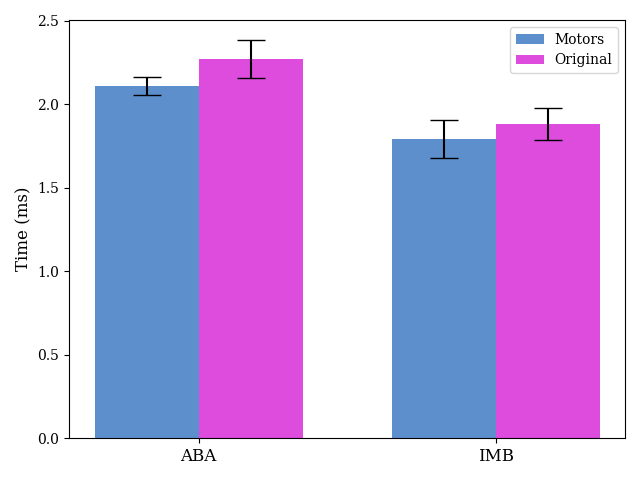
\includegraphics[width=0.65\textwidth]{Images/Results/time_comparison_aba.png}
\end{figure}

Regarding the computational performance, the modified \ac{ABA} algorithm is expected to be slower than the original one, due to the additional computations required to compute the motor dynamics. However, from the results reported in \cref{fig:fd_benchmark}, it is possible to see that the modified \ac{ABA} algorithm is comparably fast to the original one, with a difference of less than $1\%$ in the execution time. This is due to the fact that the additional computations required to compute the motor dynamics are negligible compared to the other computations performed by the algorithm.

\begin{figure}
    \centering
    \caption{Modified Forward Dynamics -- Algorithm Comparison.}
    \label{fig:fd_comparison}
    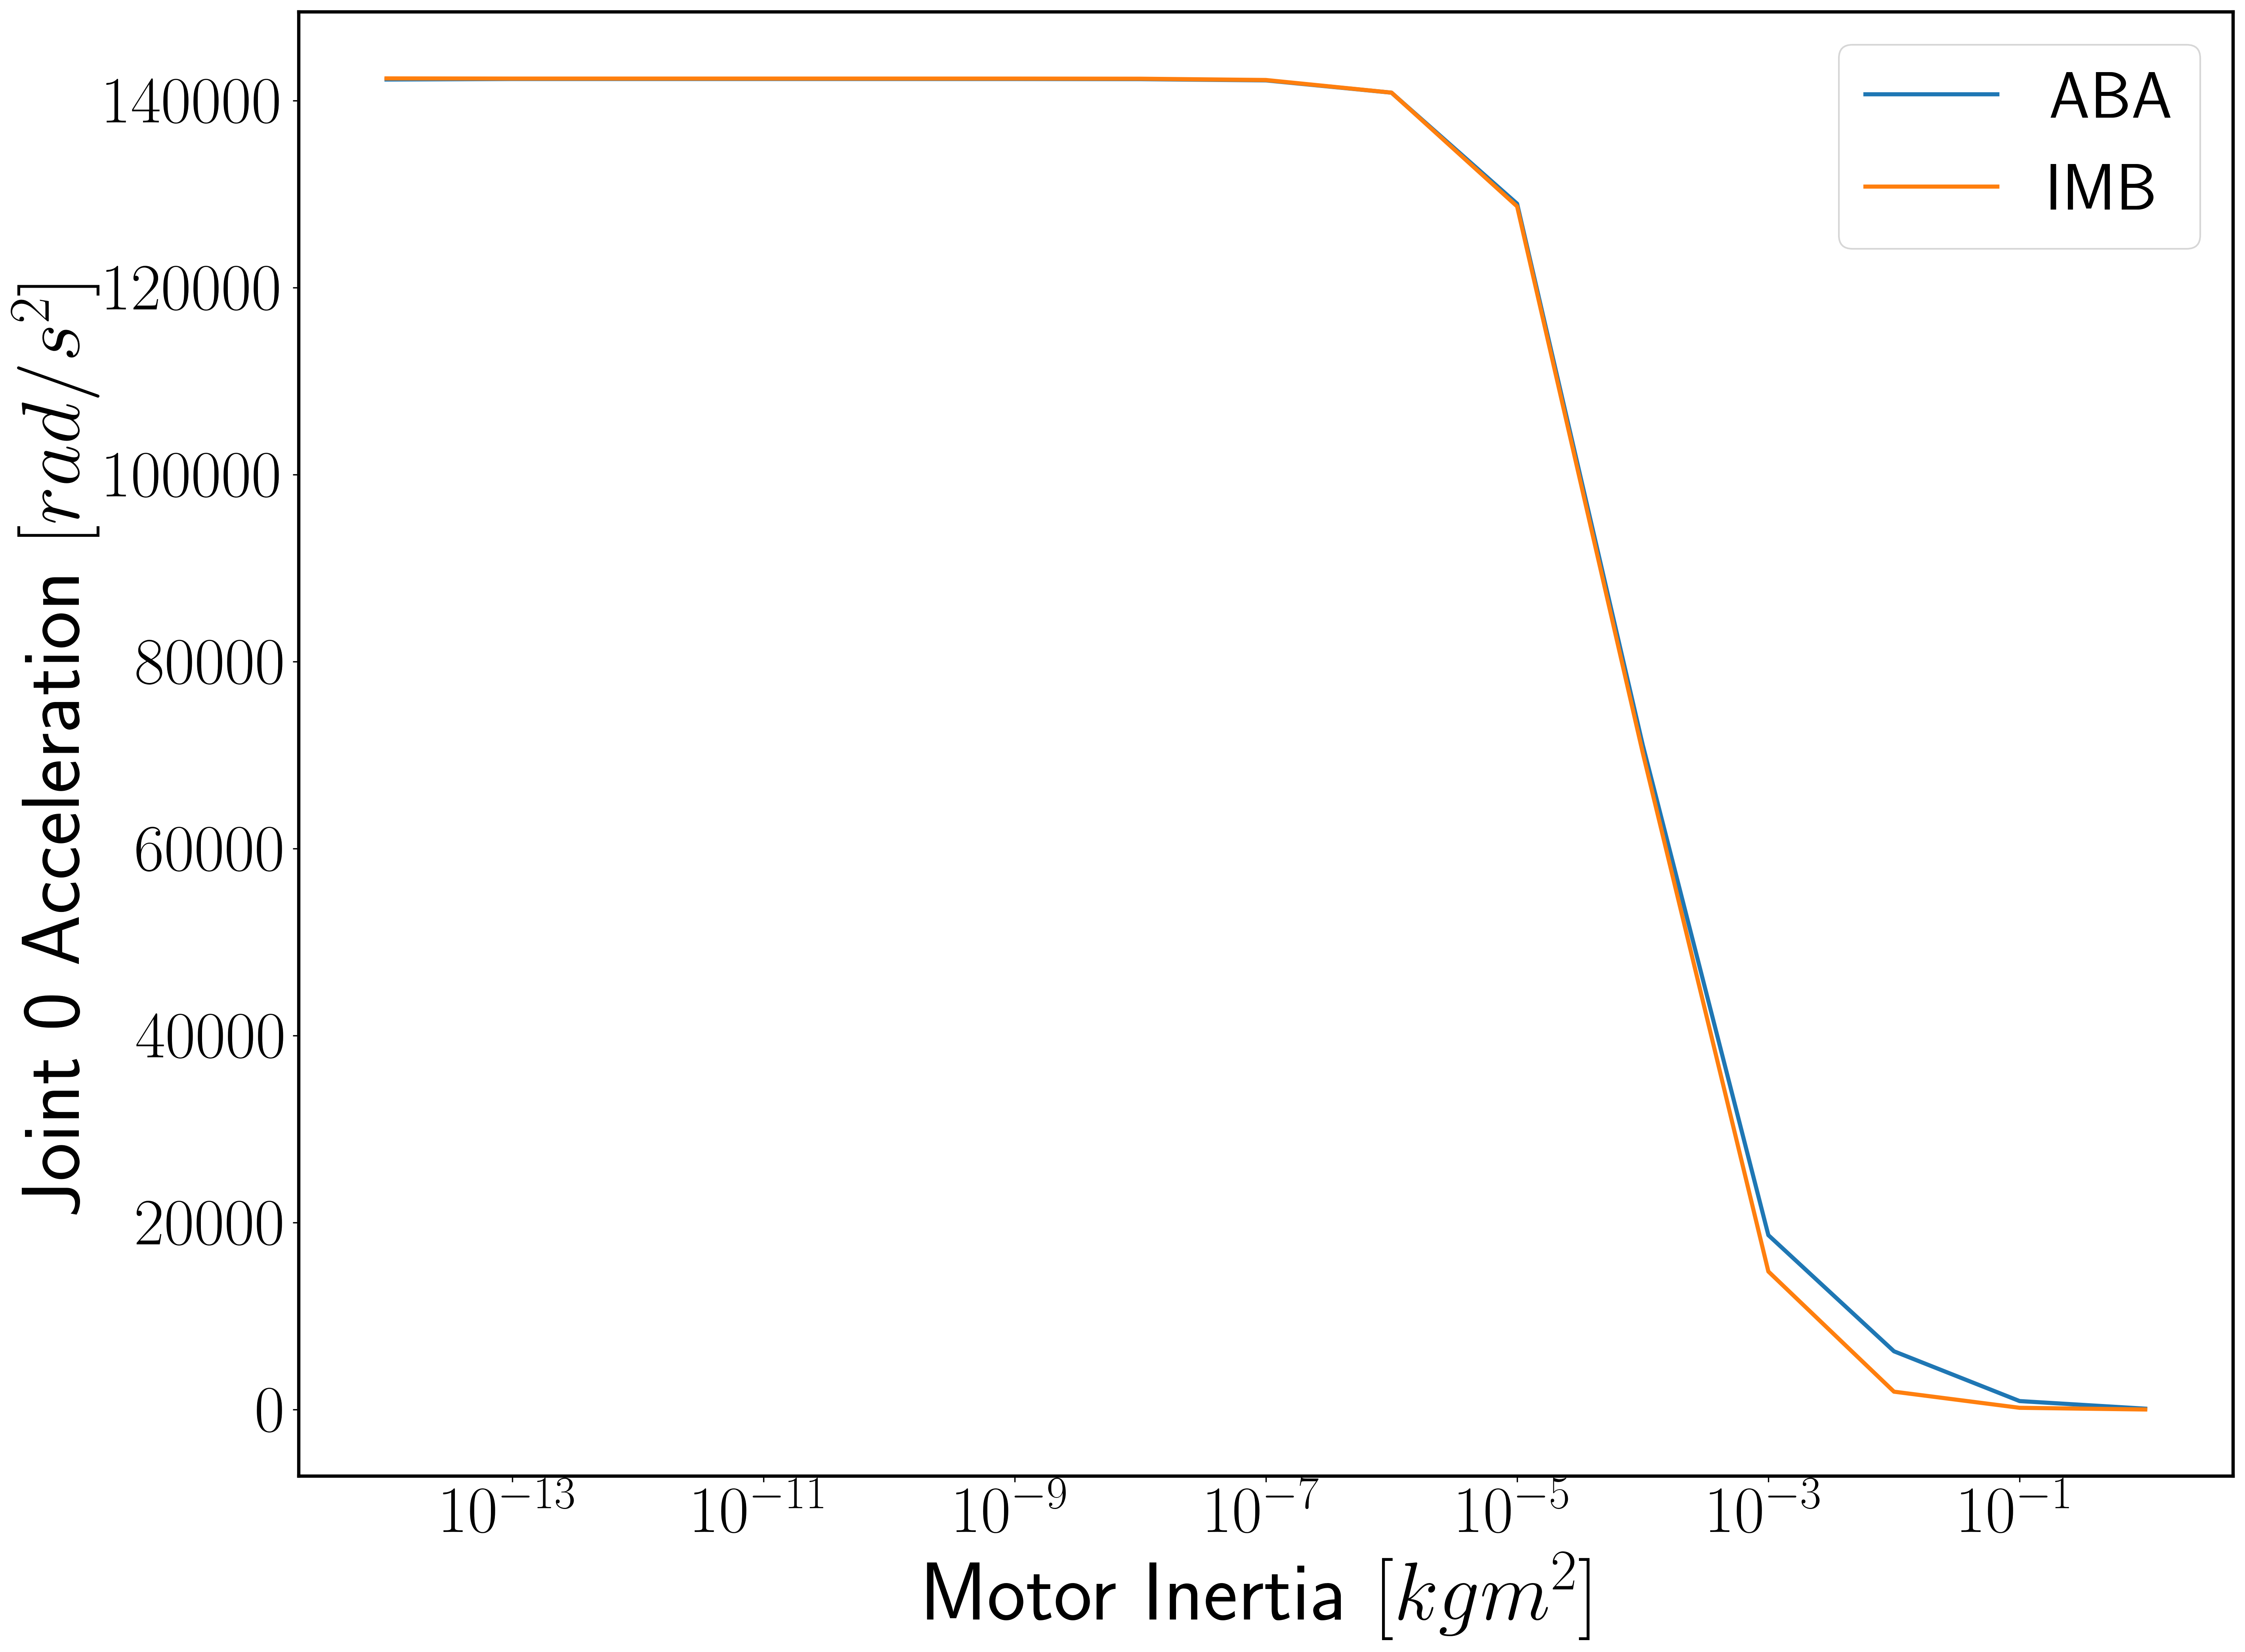
\includegraphics[width=0.6\textwidth]{Images/Results/ABA_IMB.png}
\end{figure}

When evaluating the difference between the results obtained with the modified \ac{ABA} algorithm and the modified Inertia-Matrix method, it is possible to see that the difference depends on the motor inertia values. In particular, the difference is larger for the joints with a larger motor inertia, while it is smaller for the joints with smaller motor inertia, as can be seen in \cref{fig:fd_comparison}. This is due to the fact that as the motor inertia increases, the gyroscopic effects of the spinning rotors, expressed in the algorithm as contributions on the bias forces ${}^M \mathbf{v}_i \times ^* \mathbb{I} _i ^M \mathbf{v}_i$ which is not considered in the Inertia-Matrix method, become more relevant.


\section{Robot Codesign Results}
\label{sec:codesign_results}

The usage of genetic algorithms together with reinforcement learning involves the tuning of several hyperparameters, which can have a significant impact on the performance of the algorithm. Moreover, given the computational cost of the reinforcement learning training, the choice of parameters is bounded by the available computational resources. 

As an example, the number of generations of the genetic algorithm is strictly related to the number of reinforcement learning training that can be performed, yet reducing its value can lead to a smaller explored space of solutions, bringing therefore to suboptimal results.

\begin{figure}
    \centering
    \caption{Cartpole RL Training Metrics.}
    \label{fig:cartpoleresults}
    \subfloat[Explained Variance]{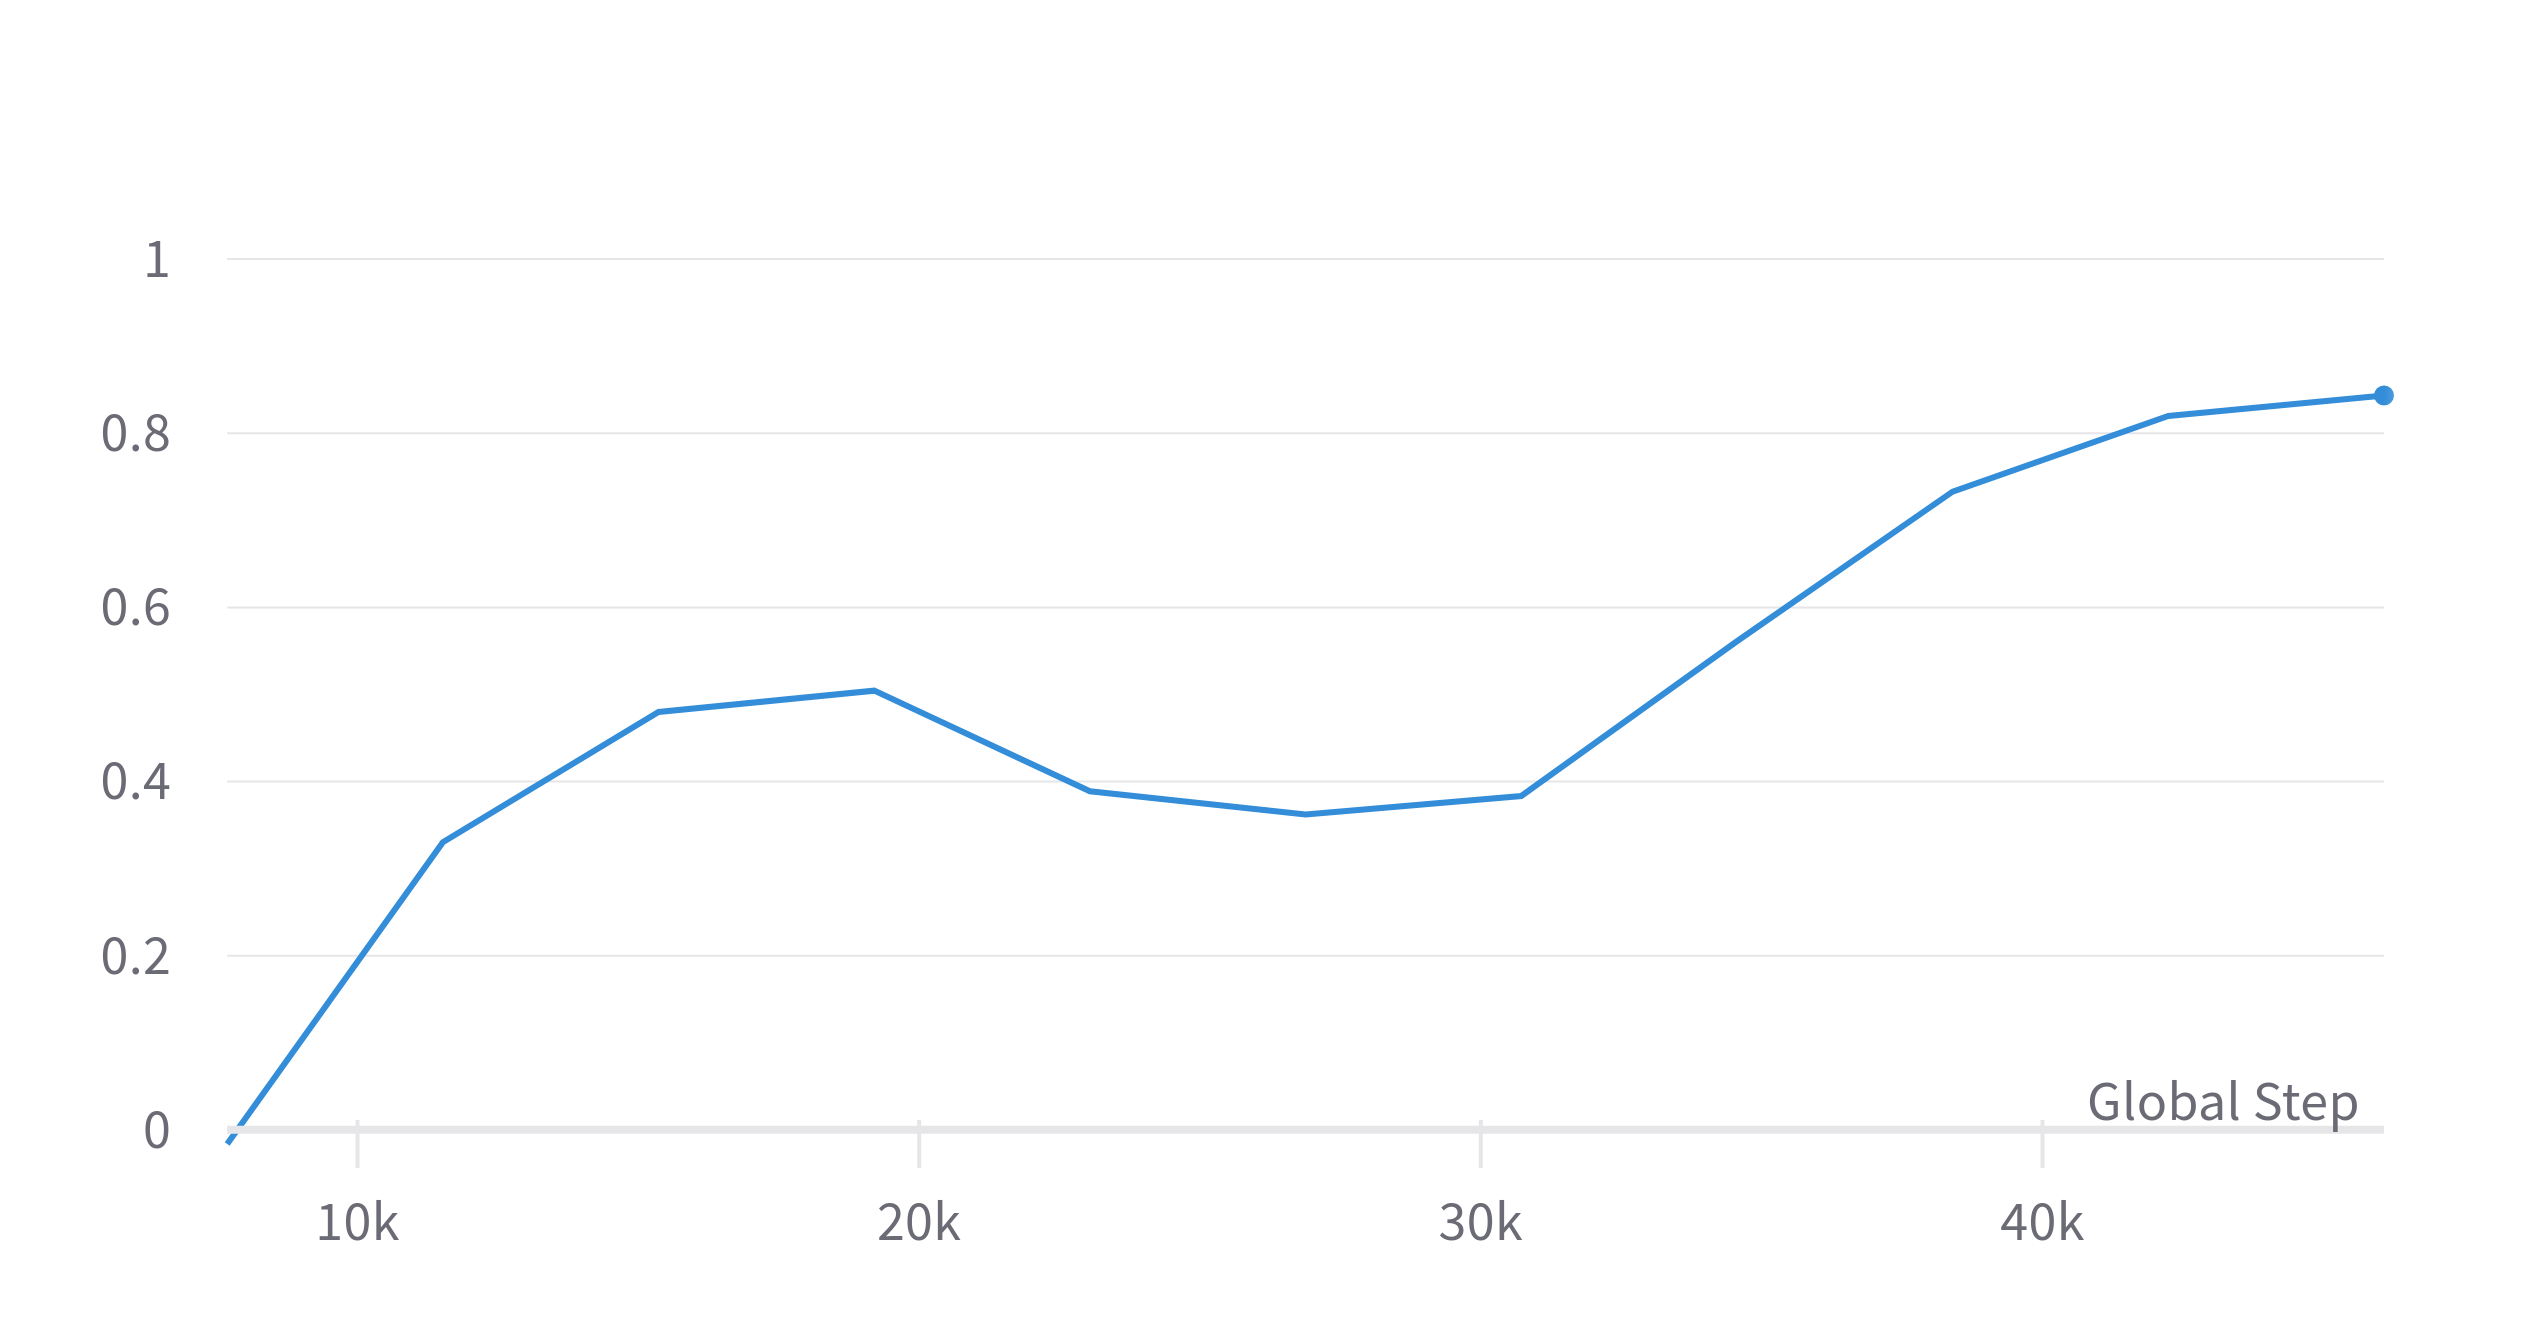
\includegraphics[width=0.48\textwidth]{Images/Results/expvariance_cartpole.png}}
    \subfloat[Approximated KL]{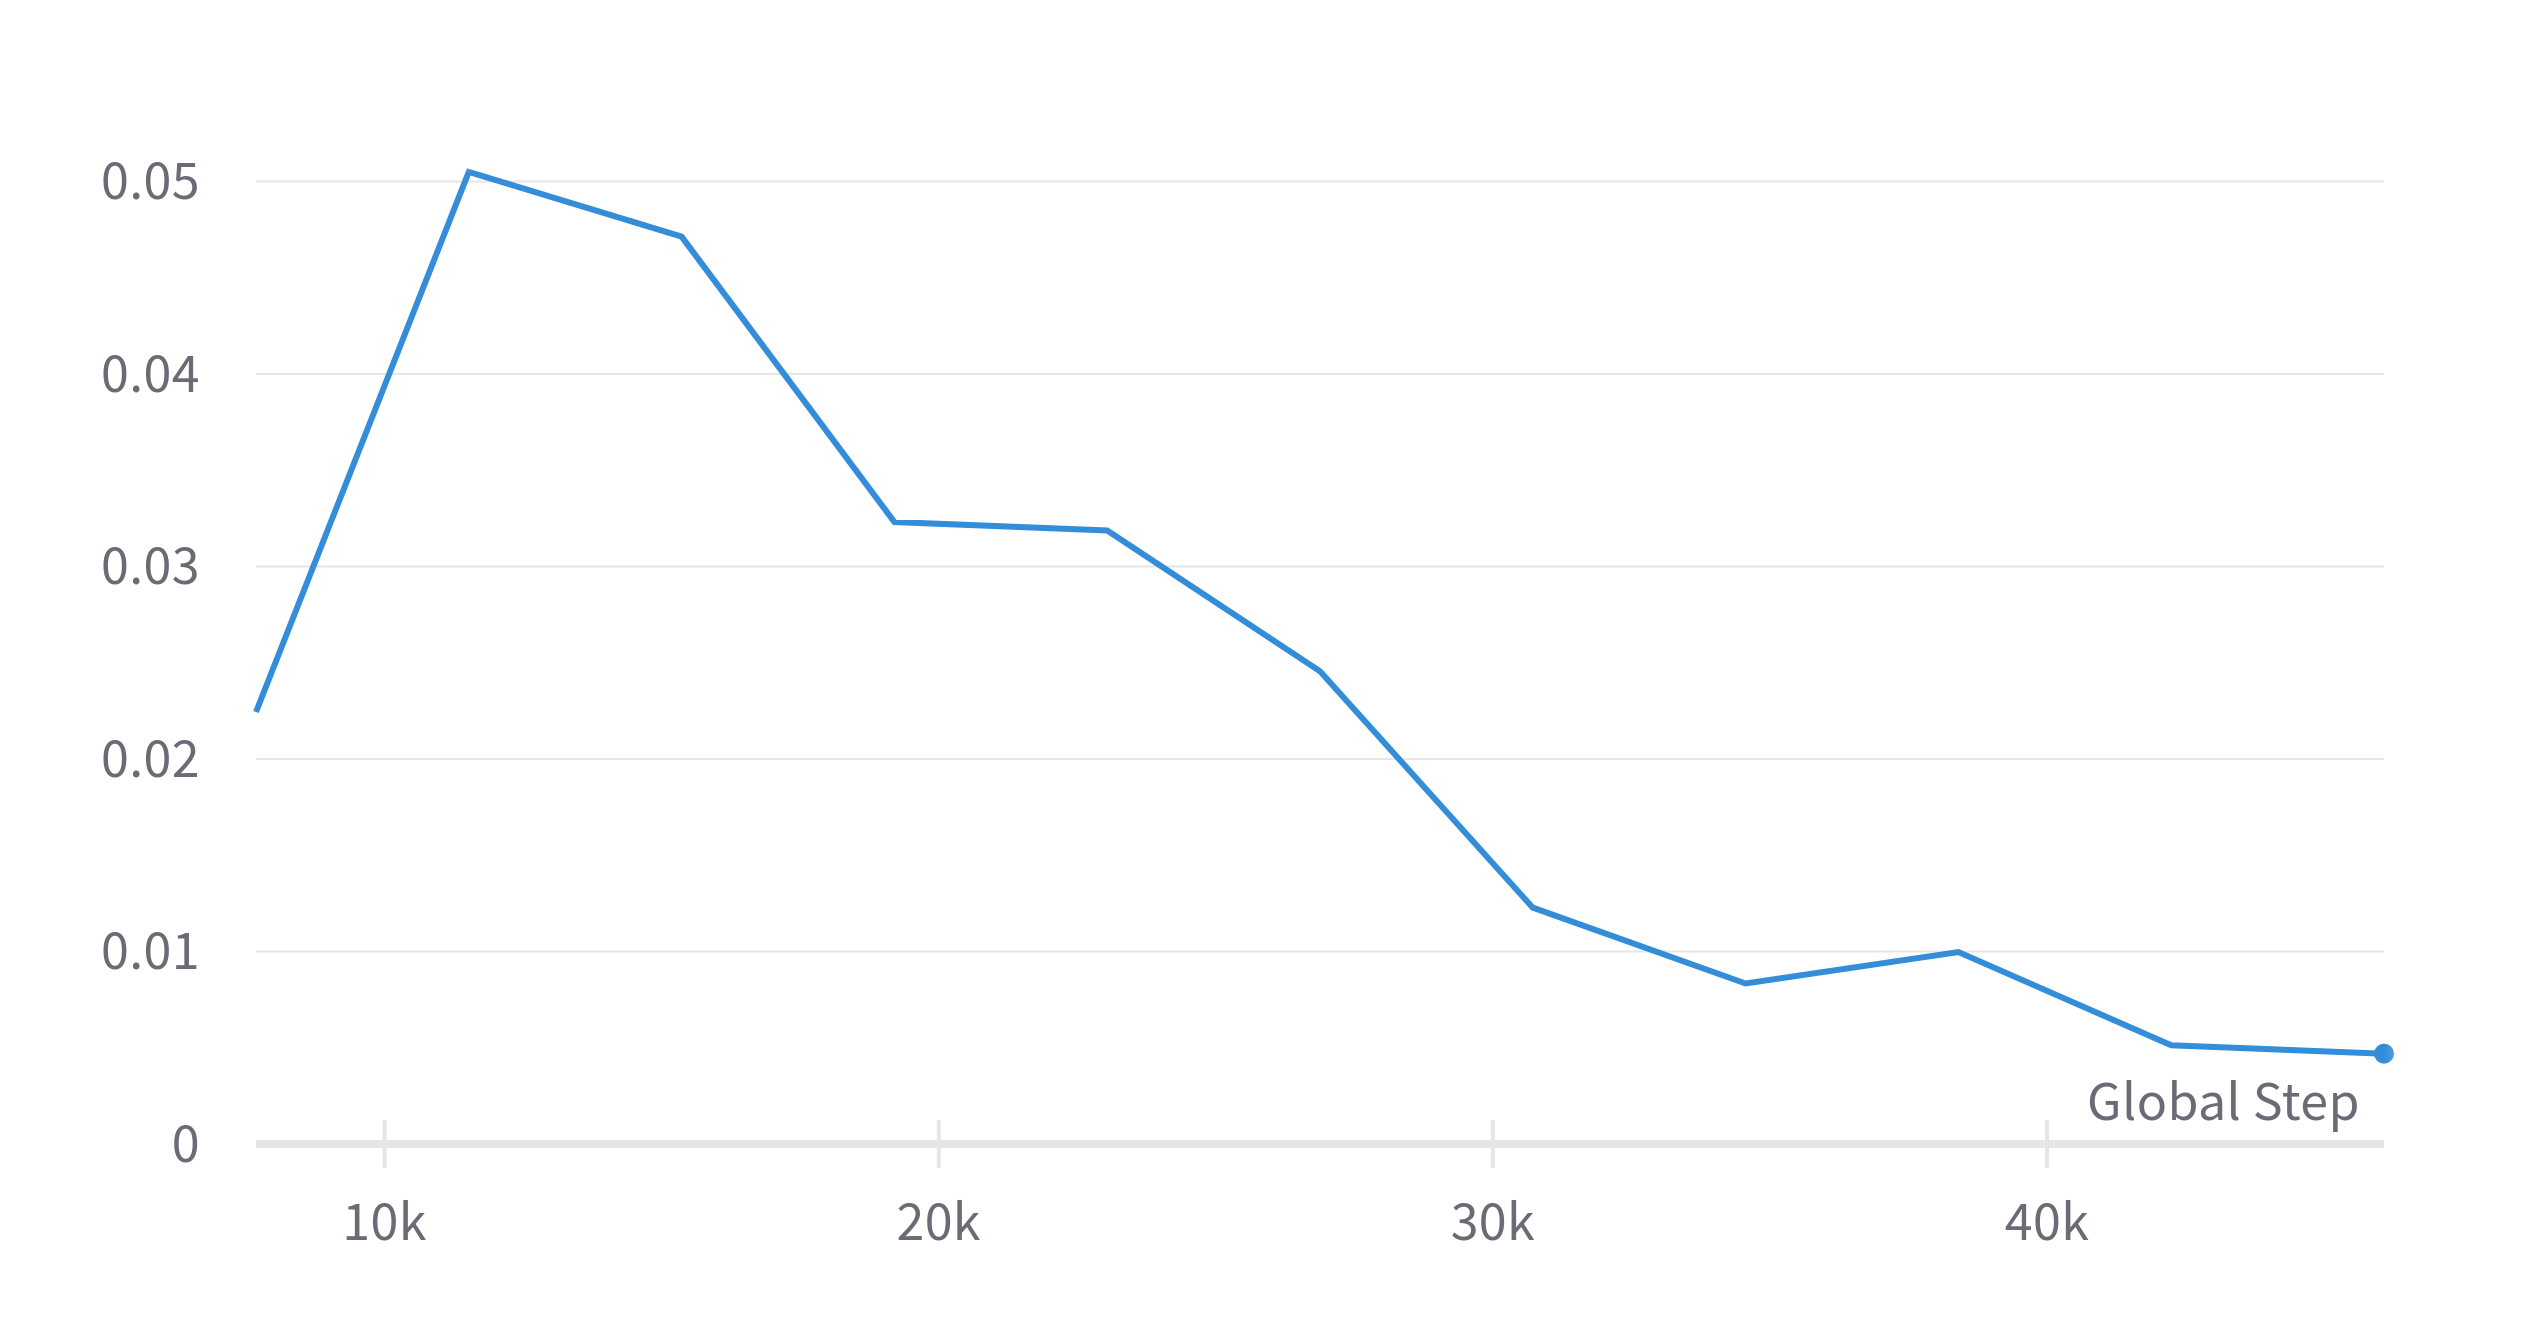
\includegraphics[width=0.48\textwidth]{Images/Results/kl_cartpole.png}} \\
    \subfloat[Value Loss]{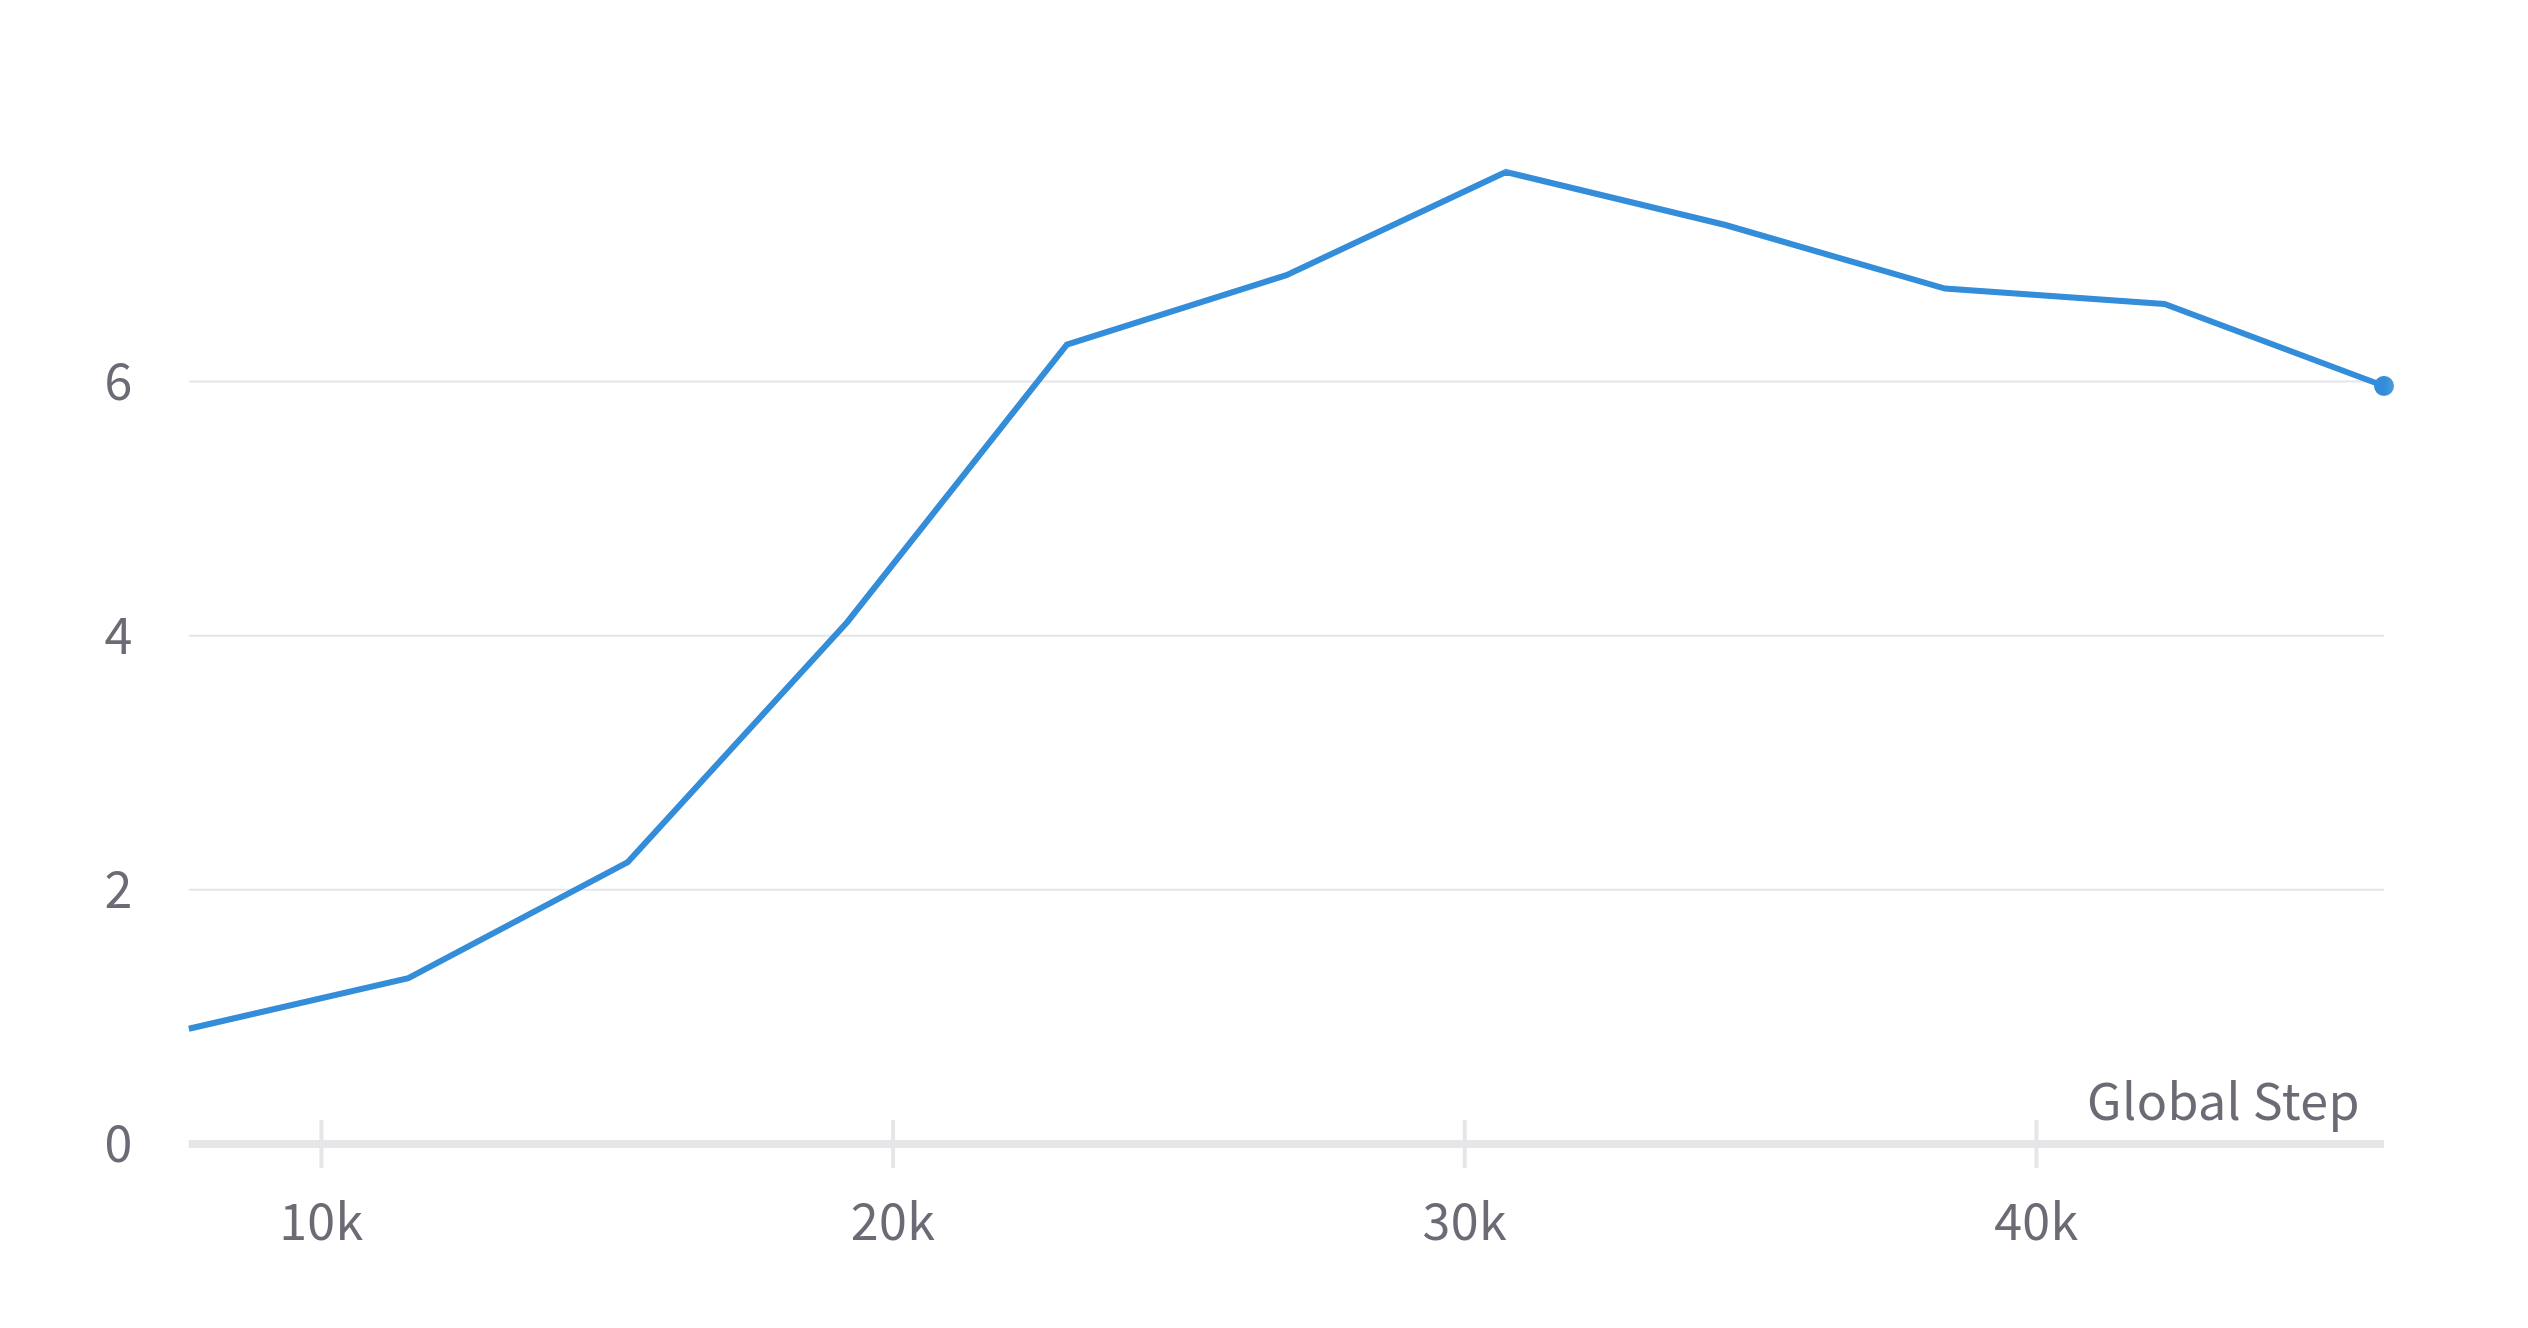
\includegraphics[width=0.48\textwidth]{Images/Results/loss_value_cartpole.png}}
    \subfloat[Rollout Metrics]{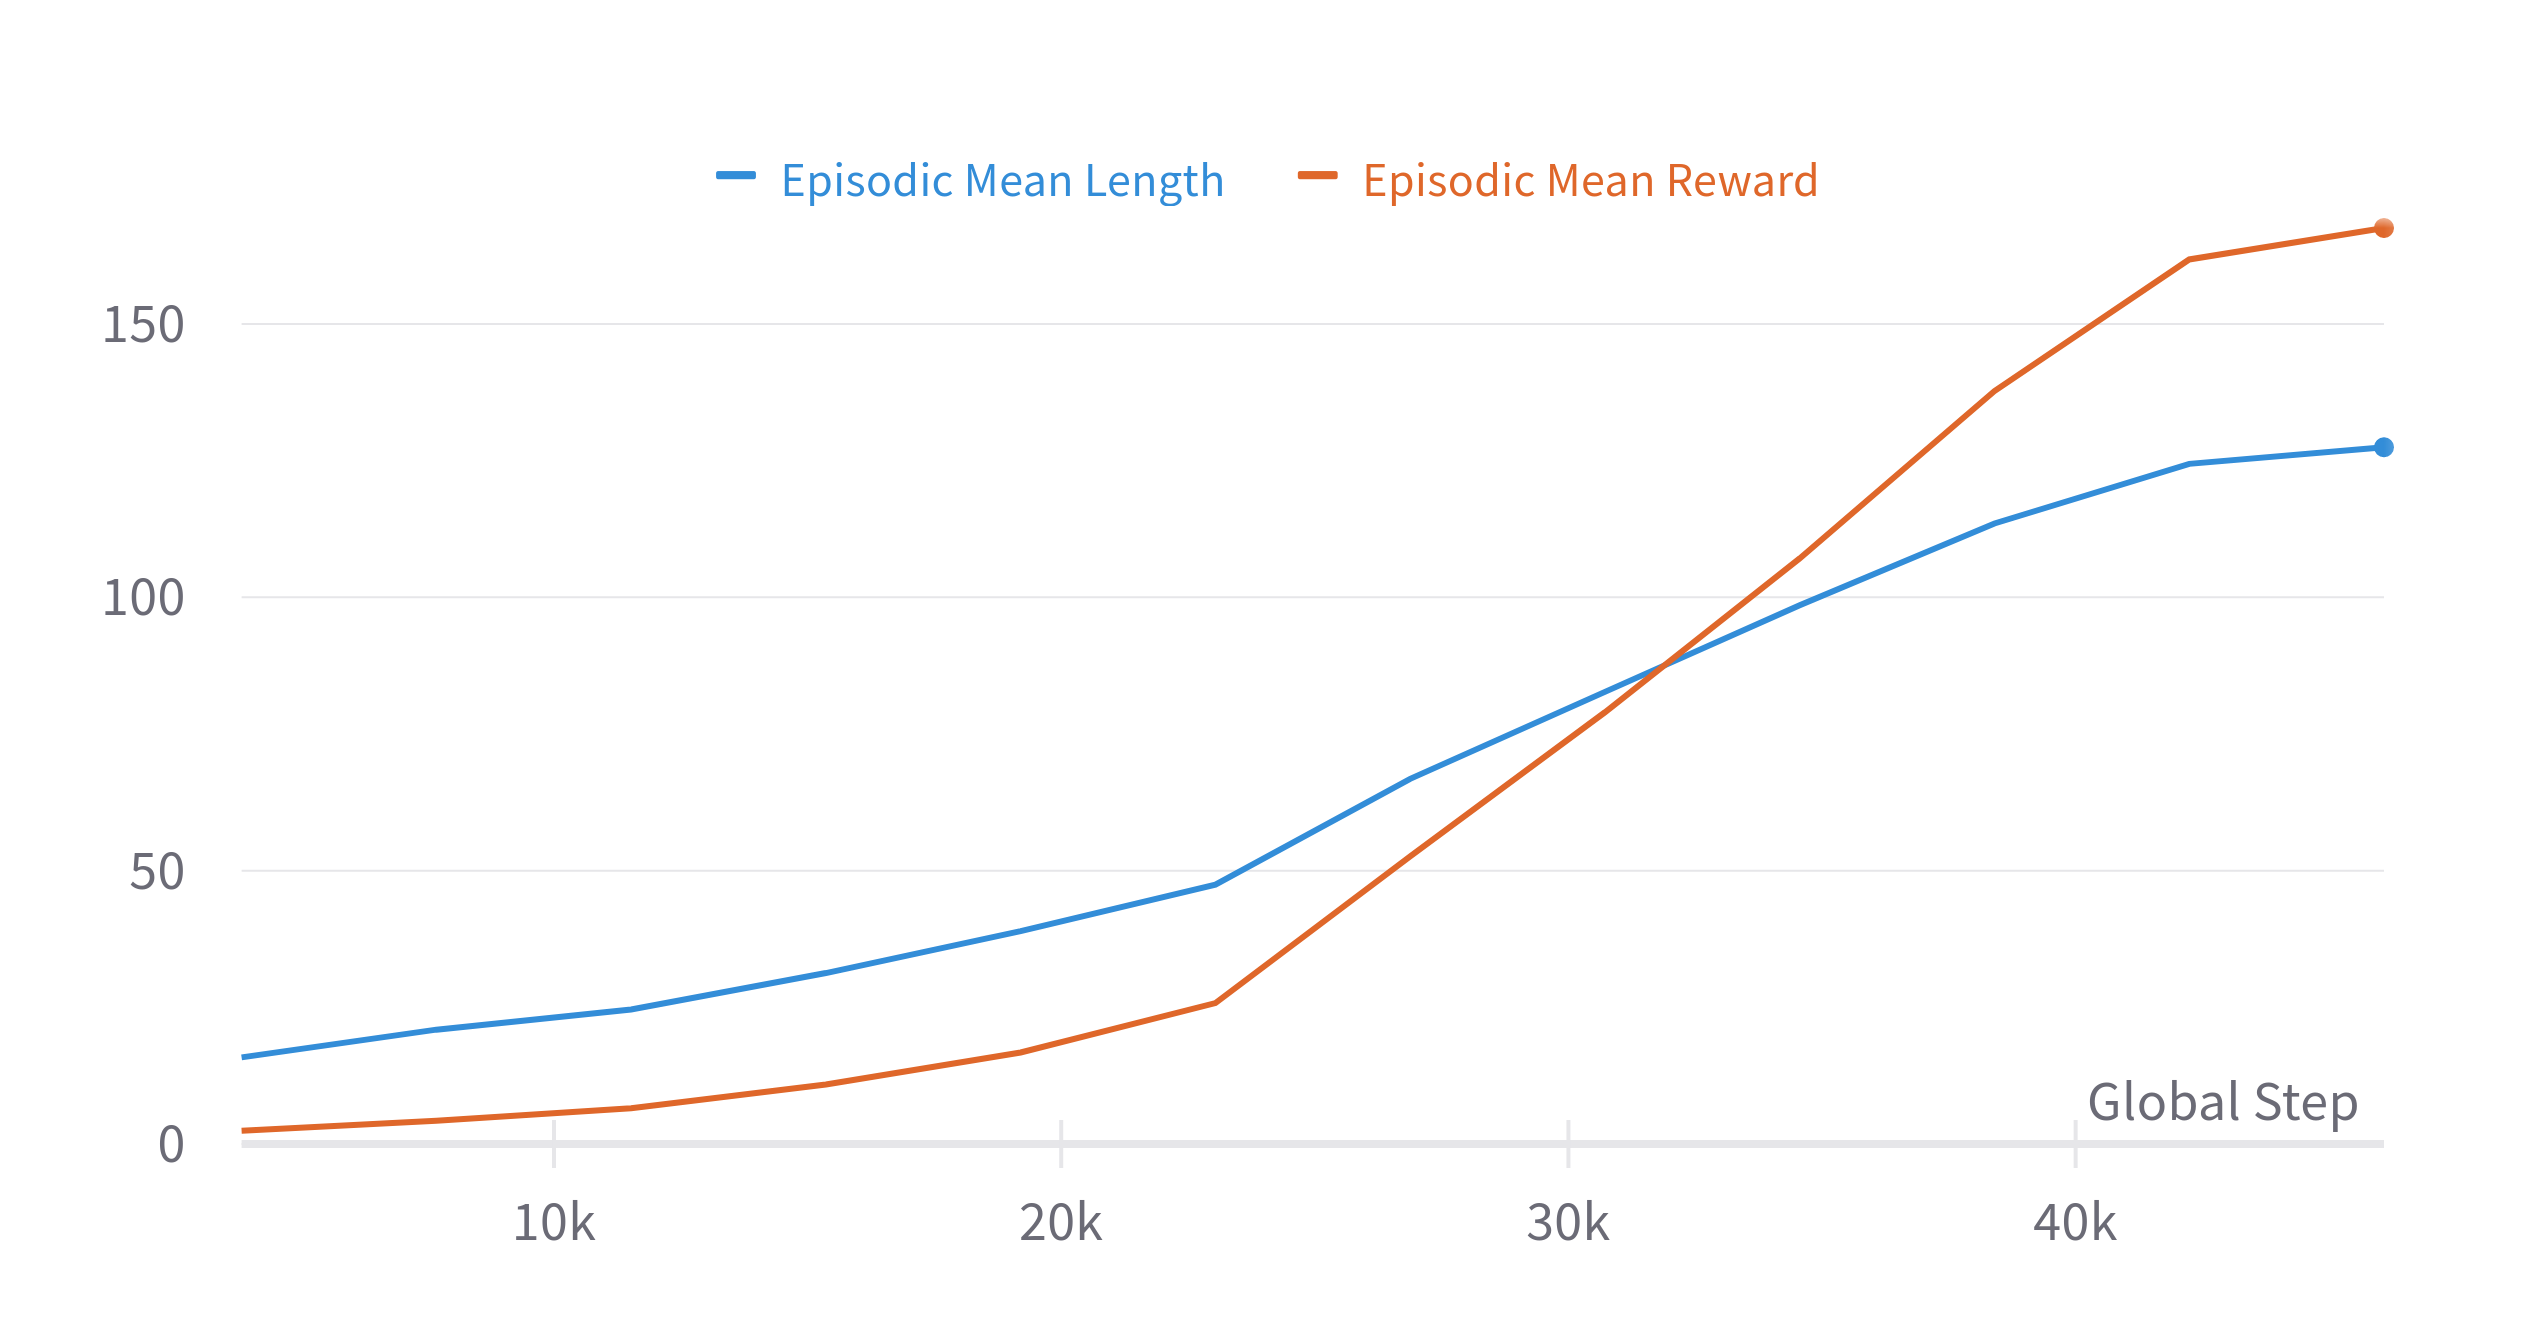
\includegraphics[width=0.48\textwidth]{Images/Results/rollout_cartpole.png}}
\end{figure}

In reinforcement learning, it is crucial to keep track of some metrics during the training, in order to evaluate the performance of the algorithm, detect possible issues, and stop the training if the maximum reward is reached. In fact, if the training does not have an early stopping condition, the agent might begin to forget the optimal policy, leading to disastrous results. With the aim of logging the training metrics, we opted for the use of \textit{Weights {\&} Biases}\footnote{\url{https://wandb.ai}}, a tool that allows for the tracking, which in opposition to the most common \textit{Tensorboard}\footnote{\url{https://www.tensorflow.org/tensorboard}} tool, supports online logging and real-time monitoring of the training metrics. The main metrics that we tracked during the training are:

\begin{itemize}
    \item \textbf{Explained Variance}: a metric that measures the proportion to which the value function is a good predictor for the returns;
    \item \textbf{Approximated KL}: a metric that measures the distance between the new policy and the old policy;
    \item \textbf{Value Loss}: a metric that measures the difference between the algorithm's expectation of a state's value and the empirically observed value of that state;
    \item \textbf{Episodic Mean Reward}: the mean reward obtained during the episode;
    \item \textbf{Episodic Mean Length}: the mean length of the episode.
\end{itemize}

Note that we are reporting the \textit{mean} episodic reward and length as we are training multiple environments in parallel. In particular, if the algorithm is converging, the explained variance should get closer to $1$, the approximated KL should remain small, the value loss should decrease and the mean reward and the mean episode length should increase or remain constant.


The results obtained during the training are reported in \cref{fig:cartpoleresults}. As expected, the explained variance gets closer to $1$ as the training progresses, while the approximated KL divergence remains small, which means that the policy update is not too large. The value loss decreases as the training progresses, which means that the value function is getting better at predicting the return. The rollout metrics show that the mean reward and the mean episode length increase as the training progresses, which means that the policy is getting better at solving the task.

For what concerns the genetic algorithm, the hyperparameters had been tuned in order to expand the search space as much as possible. As the dimensionality and the discrete nature of the problem allow us to represent the search space as a grid, we could easily verify its extension as in \cref{fig:searchspace}, in which the possible combinations for the two joints are represented in a 2D grid, and a color scale is used to represent the normalized fitness of the evaluated chromosomes.

\begin{figure}
    \centering
    \caption{Evolutionary Algorithm Explored Search Space.}
    \label{fig:searchspace}
    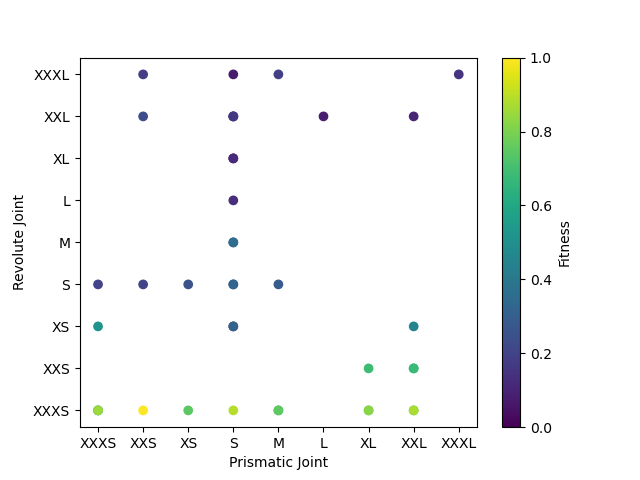
\includegraphics[width=0.7\textwidth]{Images/search_space.png}
\end{figure}

The results obtained with the genetic algorithm are reported in \cref{fig:codesignresults}. As expected, the fitness increases as the training progresses, indicating that the genetic algorithm is able to update the population with increasingly more individuals with higher fitness, as shown in \cref{fig:fitness}. Moreover, the diversity, reported in \cref{fig:diversity}, had been tracked in order to verify that the standard deviation from one generation to the other decreases, indicating a convergence of the population toward an optimal solution. Interestingly enough, the codesign framework seems to generally converge to small motors, yet for the prismatic joint, the one corresponding to the sliding cart, the chosen motor has a higher viscous friction and inertia.

\begin{figure}
    \centering
    \caption{Cartpole Codesign Results.}
    \label{fig:codesignresults}
    \subfloat[Fitness Plot \label{fig:fitness}]{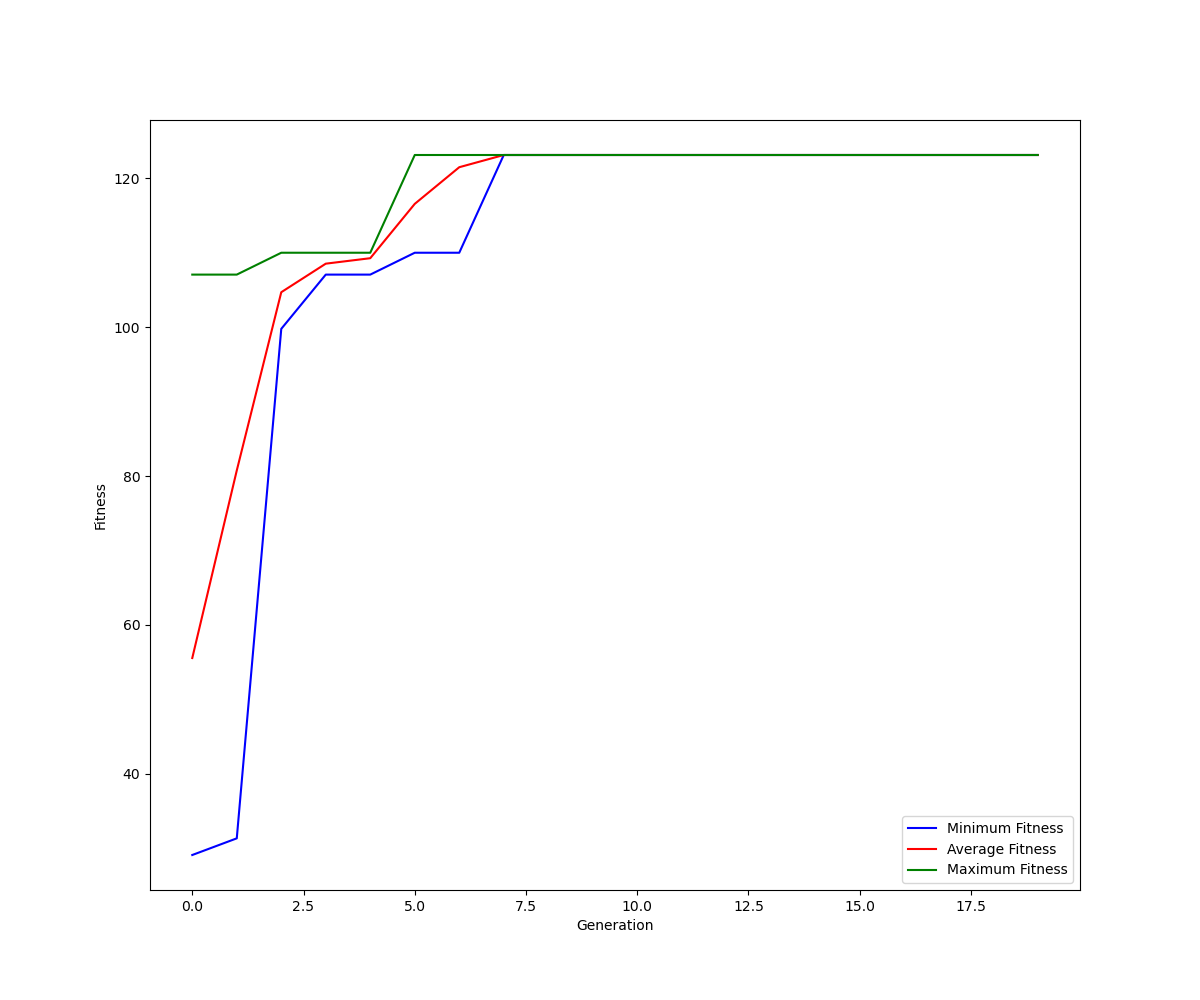
\includegraphics[width=0.49\textwidth]{Images/convergence_plot.png}}
    \subfloat[Diversity Plot \label{fig:diversity}]{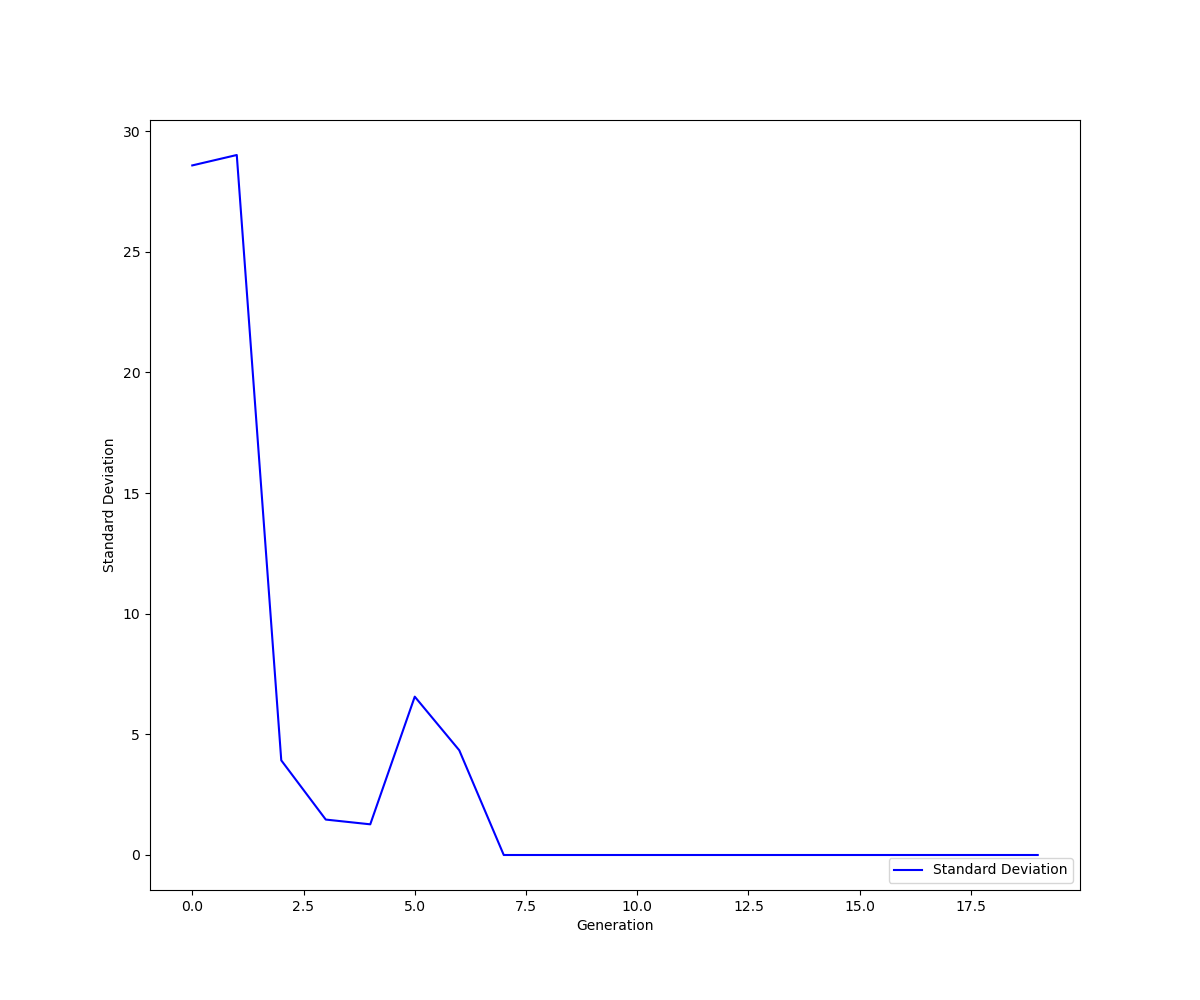
\includegraphics[width=0.49\textwidth]{Images/diversity_plot.png}}
\end{figure}
